% ===============================================================================================
% ===============================================================================================
% =====================================Conference Logistics======================================
% ===============================================================================================
% ===============================================================================================

\section{Conference Logistics}

\subsection{Date Selection}


We propose the conference be held on the following dates: 
\begin{enumerate}
	\item Thursday, April 8$^{th}$ - Sunday, April 11$^{th}$ 
	\item Thursday, April 15$^{th}$ - Sunday, April 18$^{th}$
\end{enumerate}
We believe either of these dates would serve as an appropriate first choice because they avoid major conflict dates like finals and spring break for most schools. Additionally, mid-April offers pleasant mild weather in Champaign. The reason for proposing two weekends to host the conference is due to the UIUC tradition of hosting Mom's Weekend on or near the first weekend in April. The Illinois Mom's Association has not yet announced their 2021 dates but to avoid potential conflict, we suggest two dates. In the event that both of these dates are unavailable our backup date is 
\begin{itemize}
	\item Thursday, April 1$^{st}$ - Sunday, April 4$^{th}$.  
\end{itemize}
This is a backup date because Easter falls on that Sunday. In general, this should be avoided. In this case we found that holding the conference at the end of April would conflict with finals for students and holding it earlier in March would conflict with several spring breaks as well as having potentially poorer weather. A detailed conflict schedule is listed in Appendix A. 

\subsection{Conference Facilities}


\textbf{The Illini Union}\\


% \begin{figure}[h!]
% 	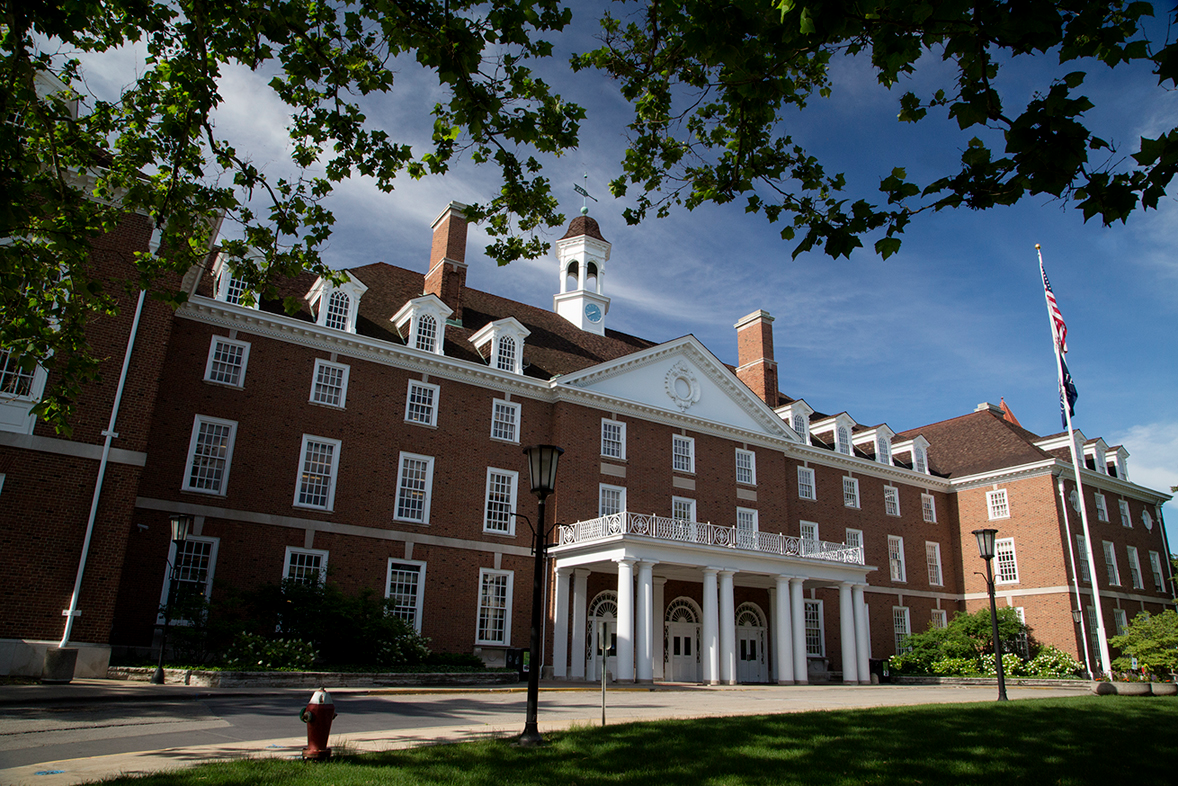
\includegraphics[width=\textwidth]{illini-union.png}
% 	\caption{Illini Student Union}
% \end{figure}



The Illini Union is capable of hosting the entire technical program. Keeping the conference contained in one convenient location while being within easy access of the rest of the campus. Technical sessions will be held in a combination of rooms on the second, third, and fourth floors of The Union. Each of these rooms has at least enough capacity for 42 people and A/V capability. There will also be rooms available to have panels and workshops during the course of the technical program. The Illini Rooms A and B will be a combined space for the career fair and Illini Room C will host the poster sessions. We will keep the space open to allow the poster sessions and career fairs to share attendance and encourage networking. A detailed list of room capacities and floor plans are located in Appendix D: Building Layout. 



\subsection{Conference Contingency Plan}
In the event that the Union has reduced availability during the conference we have the ability to host technical sessions and workshops at a combination of buildings: The National Center for Supercomputing Applications (NCSA) and Beckman Institute. These two buildings have large capacity rooms and small capacity rooms. As these buildings are UIUC property, the cost of renting them are significantly reduced compared to a private facility. Additionally, these two buildings are adjacent to one another and are at most a 10 minute walk from either the Union or Marriott TowneSuites. See Fig.\ref{fig:conf-map} for a map of the proposed conference facilities.\\


\textbf{National Center for Supercomputing Applications (NCSA)}\\
NCSA is a hub of transdisciplinary research and digital scholarship where University of Illinois faculty, staff, and students, and collaborators from around the globe, unite to address research grand challenges for the benefit of science and society.\\
\begin{figure}[H]
	\centering
	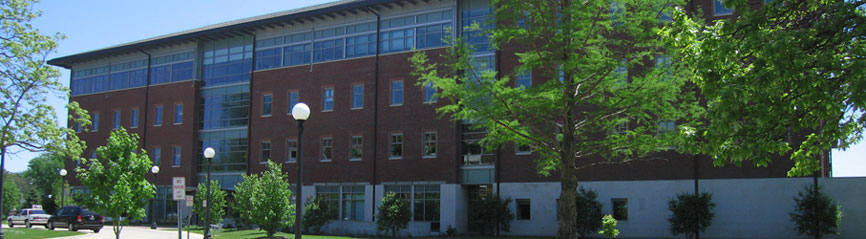
\includegraphics[width=0.8\textwidth]{ncsa_front.jpg}
	\caption{NCSA}
	\label{fig:ncsa}
\end{figure}

\textbf{Beckman Institute}
The Beckman Institute for Advanced Science and Technology at the University of Illinois is an interdisciplinary research institute devoted to leading-edge research in the physical sciences, computation, engineering, biology, behavior, cognition, and neuroscience.\\

\begin{figure}[H]
	\centering
	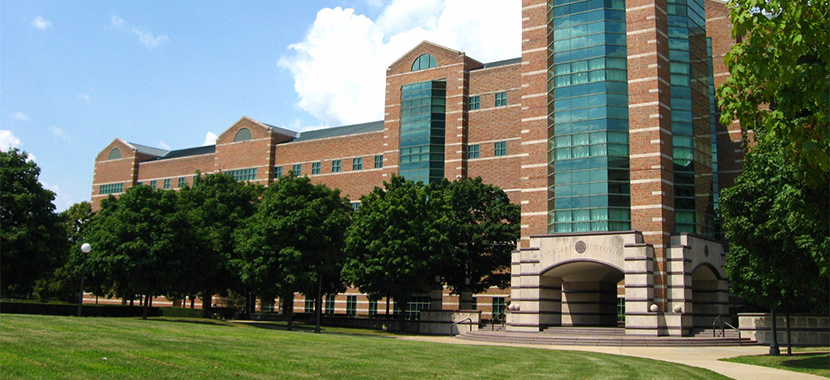
\includegraphics[width=0.8\textwidth]{beckman.jpg}
	\caption{Beckman Institute}
	\label{fig:beckman}
\end{figure}

\begin{figure}[H]
	\centering
	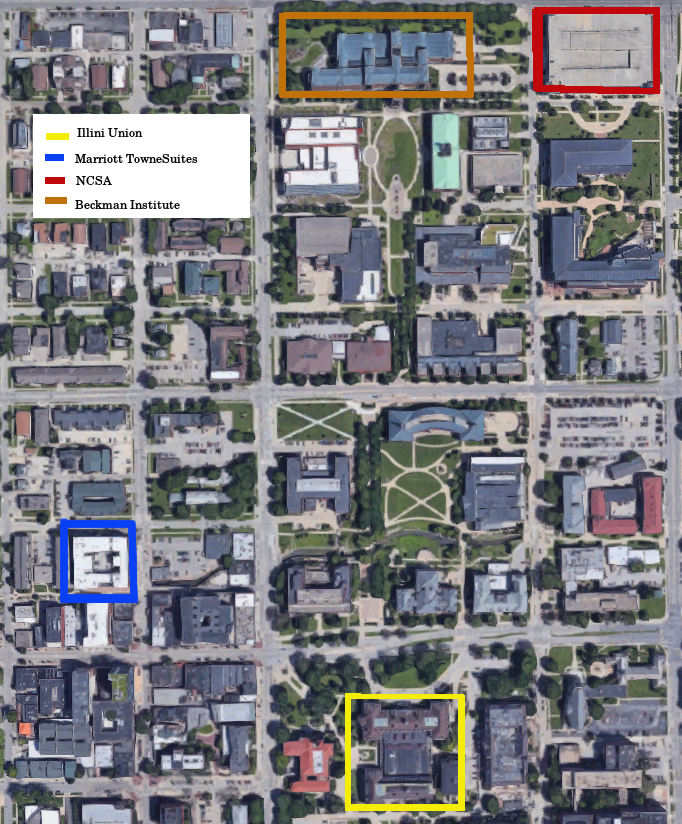
\includegraphics[width=\textwidth]{campus_map.png}
	\caption{Map of conference facilities and hotels}
	\label{fig:conf-map}
\end{figure}


\subsection{Hotels and Accommodations}

$\textbf{The Garden Hotel Urbana}$\\
When selecting the primary hotel to accommodate students we considered the ability to host all students under one roof over proximity to the conference activities. The Garden Hotel Urbana (soon to be the Radisson) will be the primary hotel for all attendees. Since this hotel is just beyond walking distance from the main conference activities, regular transportation to and from the Union will be provided during peak commuting hours (8am-10am $\&$ 3pm-5pm). Additionally, there is a CU-MTD bus stop adjacent to the hotel that travels directly to the Union and runs every 10 minutes from 8am to 6pm. This will also be the location of the opening ceremony dinner.\\ 


$\textbf{Illini Union}$\\
This is the primary hotel for invited speakers and panelists. Commuting to the conference will be as easy as taking the elevator downstairs because the Illini Union is where the primary conference activities will be held. The Union is also a five-minute walk from Green Street, the campus hub of dining and social activities. Guests have access to Wi-Fi and, upon request, guest passes to the university recreational facilities. Breakfast is provided in the form vouchers for any of the hotel restaurant options inside the Union. Hosting technical sessions, workshops, and plenaries in the Union will help us negotiate a lower room rate.\\


$\textbf{Marriott TowneSuites}$\\
In the event that attendance exceeds 600 people, we will have overflow rooms in the Marriott TowneSuites. Rooms at the Marriott resemble a studio apartment with an open floor plan, refrigerator, stove, microwave,dishes, and dining area. Many rooms are equipped with pull-out couches, allowing 5 students to share a queen double room if desired. The hotel offers internet access for a maximum of 3 devices per room. The hotel is located on Green Street and the Illini Union a mere five-minute walk away. For $\$7$ a day, guests may park in a parking garage with 8ft clearance.\\
\begin{figure}[H]
	\centering
	\begin{subfigure}{0.5\textwidth}
		\centering
		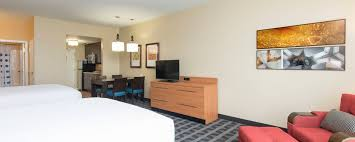
\includegraphics[width=0.9\linewidth]{marriott_room1.jpeg}
	\end{subfigure}%
	\begin{subfigure}{0.5\textwidth}
		\centering
		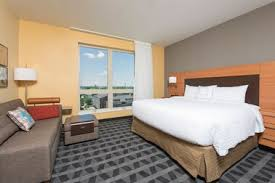
\includegraphics[width=0.9\linewidth]{marriott_room2.jpeg}
	\end{subfigure}
	\caption{Marriott Rooms: Left, a queen double. Right, a king single}		
\end{figure} 

UIUC is one of most well represented schools at past student conferences. Students from UIUC will be able to stay in their respective dorms and apartments to maximize the number of hotel rooms available to out of town guests. 

\begin{tabular}{cccccc}
\hline\hline
Hotel & Distance from the Union (mi) & Dates & Number of Rooms & Rates & Per Person\\
\hline\hline
Garden Urbana & 2.2  & 4/8-4/11 & 198 & 119 & $\$$29.75\\
Illini Union & 0.0 & 4/8-4/11 & 35 & 134 & $\$$33.5\\
\end{tabular}

\newpage
\subsection{Travel and Transportation}

\subsubsection{Getting to Champaign}
The University of Illinois is a 2.5 hour drive from one of the largest airports in the world, O'Hare International Airport. There is also a small airport located just 20 minutes outside of campus. Additionally, there is a reliable bus service, Peoria Charter, that runs between O'Hare and the UIUC campus several times per day. Below are the round-trip, non-stop, airfare costs for the first weekend of April. Peoria Charter fare from O'Hare to UIUC is currently $\$61$ round-trip.   
\begin{center}
	\begin{tabular}{lcc}
		\hline\hline
		\textbf{School} & \textbf{Departure City} & \textbf{Airfare to O'Hare (ORD)*}\\
		\hline\hline
		University of Florida & Orlando (ORL) & $\$$ 236\\
		Texas A$\&$M & College Station (CLL)& $\$$ 393\\
		Penn State University & State College (SCE) & $\$$ 349\\
		MIT & Boston (BOS) & $\$$ 217\\
		UNLV & Las Vegas (LAS) & $\$$ 308\\
		Georgia Tech & Atlanta (ATL) & $\$$ 175\\
		University of Michigan & Detroit (DTW) & $\$$ 240\\
		Oregon State University & Portland (PDX) & $\$$ 355\\
		RPI & Albany (ALB) & $\$$ 504\\
		UC Berkley & Oakland (OAK) & $\$$ 674\\
		UC Irvine & Orange County (SNA) & $\$$ 439\\
		US Naval Academy & Baltimore (BWI)& $\$$ 383\\
		University of Marlyand & Baltimore (BWI) & $\$$ 383\\
		University of Missouri-Columbia & St. Louis (STL) & $\$$ 168\\
		University of Nevada & Reno (RNO) & $\$$ 374\\
		University of New Mexico & Albuqurque (ABQ) & $\$$ 477\\
		NC State  University & Raleigh (RDU) & $\$$ 195\\
		University of Pittsburgh& Pittsburgh (PIT) & $\$$ 271\\
		Clemson University & Greenville (GSP) & $\$$ 295\\
		SC State University & Columbia (CAE) & $\$$ 365\\
		University of South Carolina & Columbia (CAE) & $\$$ 365\\
		Brigham Young University & Salt Lake City (SLC) & $\$$ 441\\
		U. Wisconsin-Madison & Madison (MSN) & $\$$ 229\\
		Colorado School of Mines & Denver (DEN)& $\$$ 223\\
		University of  Tennessee-Knoxville & Knoxville (TYS) & $\$$ 279\\
		Virginia Commonwealth University & Richmond (RIC) & $\$$ 326 \\
		Iowa State University & Des Moines (DSM) & $\$$ 199 \\
		University of Iowa & Cedar Rapids (CID) & $\$$ 249 \\
	\end{tabular}	
\end{center}
\textbf{*}\textit{These fares are predicted to go down around February and March.}\\

Due to the central location of UIUC, driving might be a good option for some schools and individuals. Below are the approximate driving times from several universities. 
\begin{center}
	\begin{tabular}{l r}
	\hline\hline
	\textbf{School}& \textbf{Drive Time}\\
	\hline\hline
	U. Tennessee Knoxville & 7 h 13 min\\
	University of Michigan & 5 h 24 min\\
	Clemson University & 10 h 5 min\\
	U. Missouri-Columbia & 4 h 18 min\\
	Georgia Tech University & 8 h 54 min \\
	University of Pittsburgh & 7 h 19 min\\
	U. Wisconsin-Madison & 3 h 53 min \\
	Penn State University & 9 h 17 min\\
	University of South Carolina& 10 h 44 min\\
	Iowa State University & 5 h 24 min \\
	University of Iowa & 3 h 34 min\\
	Vanderbilt University & 5 h 18 min\\
	\end{tabular}
\end{center}

\subsubsection{Getting to the Conference}
The primary location for all conference events is the Illini Union. This is also the primary hotel for conference attendees. The secondary hotel, Marriott TowneSuites is merely a five minute walk from the Union. 